\documentclass[12pt]{article}
\usepackage[top=1in, bottom=1in, left=1in, right=1in]{geometry}

\usepackage{setspace}
\onehalfspacing

\usepackage{amssymb}
%% The amsthm package provides extended theorem environments
\usepackage{amsthm}
\usepackage{epsfig}
\usepackage{times}
\renewcommand{\ttdefault}{cmtt}
\usepackage{amsmath}
\usepackage{graphicx} % for graphics files

% Draw figures yourself
\usepackage{tikz} 

% writing elements
\usepackage{mhchem}

% The float package HAS to load before hyperref
\usepackage{float} % for psuedocode formatting
\usepackage{xspace}

% from Denovo Methods Manual
\usepackage{mathrsfs}
\usepackage[mathcal]{euscript}
\usepackage{color}
\usepackage{array}

\usepackage[pdftex]{hyperref}
\usepackage[parfill]{parskip}

% math syntax
\newcommand{\nth}{n\ensuremath{^{\text{th}}} }
\newcommand{\ve}[1]{\ensuremath{\mathbf{#1}}}
\newcommand{\Macro}{\ensuremath{\Sigma}}
\newcommand{\rvec}{\ensuremath{\vec{r}}}
\newcommand{\vecr}{\ensuremath{\vec{r}}}
\newcommand{\omvec}{\ensuremath{\hat{\Omega}}}
\newcommand{\sigs}{\ensuremath{\Sigma_s(\rvec,E'\rightarrow E,\omvec'\rightarrow\omvec)}}
\newcommand{\el}{\ensuremath{\ell}}
\newcommand{\sigso}{\ensuremath{\Sigma_{s,0}}}
\newcommand{\sigsi}{\ensuremath{\Sigma_{s,1}}}
%---------------------------------------------------------------------------
%---------------------------------------------------------------------------
\begin{document}
\begin{center}
{\bf NE 250, F15\\
September 23, 2015 
}
\end{center}

% 2013-10-01

Recall the one-group diffusion equation:

\begin{equation*}
\frac{1}{v_1}\frac{\partial \phi_1(\rvec,t)}{\partial t} = S_1(\rvec,t) - 
\Sigma_{a,1}(\rvec)\phi_1(\rvec,t) + \nabla\cdot[D_1(\rvec)\nabla\phi_1(\rvec,t)]
\end{equation*}

Now, assume that space and energy dependence of the flux can be separated:

\begin{equation*}
\phi(\vecr,E,t) = \phi(\vecr,t)\psi(E), 
\text{ where $\psi(E)$ is the neutron spectrum and $\int_0^{\infty}dE\psi(E) = 1$.}
\end{equation*}

Focusing on the spatial dependence of the flux, we'll assume a homogeneous, steady-state, one-group system.

\begin{equation*}
\frac{1}{v}\frac{\partial\phi(\rvec,t)}{\partial t} = S(\rvec,t) - \Sigma_s(\rvec)\phi(\rvec,t)
+ \nabla\cdot[D(\rvec)\nabla\phi(\rvec,t)]
\end{equation*}

Steady-state: $\frac{1}{v}\frac{\partial\phi(\rvec,t)}{\partial t} = 0$


Homogeneous: no material dependence on position; 
$\Sigma_a(\rvec)\rightarrow\Sigma_a, D(\rvec)\rightarrow D$


This gives us
%
%\begin{equation*}
%0 = S(\vecr) - \Sigma_a\phi(\vecr) + D\nabla^2\phi(\vecr)
%\end{equation*}
%
%which can be rewritten as
%
\begin{equation*}
\nabla^2\phi(\vecr) - \frac{1}{L^2}\phi(\rvec) = -\frac{S(\rvec)}{D},
\text{ where $L = \sqrt{\frac{D}{\Sigma_a}} =$ diffusion length.}
\end{equation*}

%\begin{equation*}
%L = \sqrt{\frac{\langle r^2\rangle}{6}}, \langle r^2\rangle 
%=\text{ root mean square distance from birth to absorption}
%\end{equation*}

Now, consider a plane source of strength $S_0$ in an infinitely absorbing medium.

\begin{equation*}
\phi(\rvec) = \phi(x)
\end{equation*}

\begin{equation*}
\frac{d^2\phi(x)}{dx^2} - \frac{1}{L^2}\phi(x) = -\frac{S_0\delta(x)}{D}
\end{equation*}
The boundary conditions we'd like to enforce are that the source is zero other than at the plane, so within $\epsilon \rightarrow 0$:
%
\[-D \frac{d \phi}{dx}|_{+\epsilon} + D \frac{d \phi}{dx}|_{-\epsilon} = 
J_x(0^+) - J_x(0^-) = S_0\:.\]
%
We can use this to examine two sets of equations and boundary conditions.


For $x < 0$, $\frac{d^2\phi}{dx^2} - \frac{1}{L^2}\phi(x) = 0$.

Boundary conditions: 
$\lim\limits_{x\rightarrow 0^+}\vec{J}(x) = \frac{S_0}{2}, \: \lim\limits_{x\rightarrow +\infty}|\phi(x)|<\infty, \: \phi(x) \geq 0$

For $x > 0$, \: $\frac{d^2\phi}{dx^2} - \frac{1}{L^2}\phi(x) = 0$.

Boundary conditions: 
$\lim\limits_{x\rightarrow 0^-}\vec{J}(x) = -\frac{S_0}{2}, \lim\limits_{x\rightarrow -\infty}|\phi(x)|<\infty, \phi(x) \geq 0$

With the above equations and boundary conditions, we have a general solution form of

\begin{equation*}
\phi(x) = c_1e^{-x/L} + c_2e^{x/L}.
\end{equation*}

From the finite flux condition, $c_2 = 0$. Then, $\phi(x) = c_1e^{-x/L}$.

\begin{equation*}
\lim\limits_{x\to 0^+} \vec{J}(x) = \lim\limits_{x\to 0^+}\left(\frac{D}{L}c_1e^{-x/L}\right) = 
\frac{D}{L}c_1 = \frac{S_0}{2}
\end{equation*}

\begin{equation*}
c_1 = \frac{S_0 L}{2D}
\end{equation*}

\begin{equation*}
\phi(x) = \frac{S_0L}{2D}e^{-x/L}
\end{equation*}
The neutron flux falls off exponentially as one moves away from the source plane with a characteristic decay length of $L$. This holds fairly well as long as we're not too near the source and the medium is not too strongly absorbing.

------------------------------------\\
Now, consider an infinite plane centered in a slab of finite thickness $a$, surrounded by a vacuum.


For $x > 0$, $\frac{d^2\phi}{dx^2} - \frac{1}{L^2}\phi(x) = 0$.


Boundary conditions: 
$\lim\limits_{x\rightarrow 0^+}\vec{J}(x) = \frac{S_0}{2}, \: \phi(\tfrac{\tilde{a}}{2}) = 0$

For $x < 0$, $\frac{d^2\phi}{dx^2} - \frac{1}{L^2}\phi(x) = 0$.

Boundary conditions: 
$\lim\limits_{x\rightarrow 0^-}\vec{J}(x) = -\frac{S_0}{2}, \: \phi(-\tfrac{\tilde{a}}{2}) = 0$

\begin{gather*}
\phi(x) = c_1e^{-x/L} + c_2e^{x/L} \\
\text{or (which we could have also done before)} \\
\phi(x) = c_1\cosh(\tfrac{x}{L}) + c_2\sinh(\tfrac{x}{L})
\end{gather*}
%
You can use the boundary conditions to reach the full solution.


% 2013-10-03
-------------------\\
Now, consider a uniformly distributed source of strength $S_0 \tfrac{n}{cm^3s}$ within a finite slab of
width $a$ with vacuum boundaries.

\begin{equation*}
\frac{d^2\phi(x)}{dx^2} - \frac{1}{L^2}\phi(x) = -\frac{S_0}{D}
\end{equation*}

\begin{equation*}
\phi(x) = c_1e^{-x/L} + c_2e^{x/L} + \frac{S_0L^2}{D}
\end{equation*}

Boundary conditions: $\phi(\pm\tfrac{\tilde{a}}{2}) = 0$


Alternative boundary condition: $\frac{d\phi(x)}{dx}\Bigr|_{x = 0} = 0$ (symmetry)


Now, consider a uniform source in a reflected slab, where region 2 contains the source and 1 and 3 are reflectors (high scattering compared to absorption):

\begin{center}
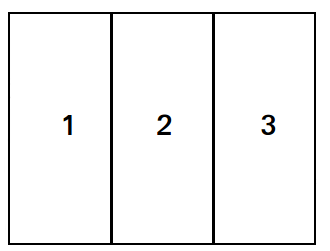
\includegraphics[height=2.5 in]{../figs/ref_slab}
\end{center}

\begin{equation*}
\frac{d^2\phi_2(x)}{dx_2^2} - \frac{1}{L_2^2}\phi_2(x) = -\frac{S_0}{D_2}, \quad -\tfrac{a}{2}<x<\tfrac{a}{2}
\end{equation*}

Boundary conditions (where subscript indicates region number):

\begin{gather*}
\phi_2(\tfrac{a}{2}) = \phi_3(\tfrac{a}{2}) \\
\vec{J}_2(\tfrac{a}{2}) = \vec{J}_3(\tfrac{a}{2}) \\
\phi_1(-\tfrac{a}{2}) = \phi_2(-\tfrac{a}{2}) \\
\vec{J}_1(-\tfrac{a}{2}) = \vec{J}_3(-\tfrac{a}{2}) 
\end{gather*}

\begin{equation*}
\frac{d^2\phi_1(x)}{dx_1^2} - \frac{1}{L_1^2}\phi_1(x) = 0, \quad -\infty<x<-\tfrac{a}{2}
\end{equation*}

\begin{equation*}
\frac{d^2\phi_3(x)}{dx_3^2} - \frac{1}{L_3^2}\phi_3(x) = 0, \quad \tfrac{a}{2}<x<\infty
\end{equation*}

Boundary conditions: 
$\lim\limits_{x\to-\infty}|\phi_1(x)| <\infty, \quad \lim\limits_{x\to\infty}|\phi_3(x)| < \infty$

----------------------\\
What if we want to solve a \textbf{generic diffusion problem}?

\begin{equation*}
D\nabla^2\phi(\rvec) - \Sigma_a\phi(\rvec) = -S(\rvec)
\end{equation*}

Working in 1D:

\begin{equation*}
M\phi(x) = f(x)
\end{equation*}
%
where $M$ is non-homogenous differential operator of order \emph{n} on a differential equation:
%
\begin{align*}
a_0(x)\phi^{(n)}(x) &+ a_1(x)\phi^{(n-1)}(x) + \dotsc + a_n(x)\phi(x) = f(x)\\
&\text{for example}\\
M = \frac{d^2}{dx^2} &- \frac{1}{L}
\end{align*}

One solution method is \textit{variation of constants / parameters}, where we break the solution into homogeneous and particular portions:
\begin{align*}
M\phi_{homog}(x) &= 0 \\
M \phi_{part} &= rhs \\
\phi(x) &= \phi_{homog}(x) + \phi_{part}(x)
\end{align*}
%
We solve the homogeneous part to yield
\[\phi_{i,h}(x),  \:i = 1,\dotsc, n \:\text{ independent solutions}\]
%
and we also know
\[\phi_{part}(x) = \sum_{i=1}^n c_i\phi_{i,h}(x)\]
%
where $c_i = c_i(x)$ and are differentiable functions that satisfy the conditions
\[\sum_{i=1}^n c'_i(x) \phi^{(j)}_{i,h}(x) = 0, \quad j = 0, \dots, n-1 \:.\]
%https://en.wikipedia.org/wiki/Variation_of_parameters

If 
\begin{align*}
\sum_{i=1}^n c_i'\phi_{i,h}(x) &= 0 \\
\sum_{i=1}^n c_i'\phi^{(1)}_{i,h}(x) &= 0 \\
&\vdots\\
\sum_{i=1}^n c_i'\phi^{(n-2)}_{i,h}(x) &= 0 \\
&\text{then} \\
\sum_{i=1}^n c_i'\phi^{(n-1)}_{i,h}(x) &= \frac{f(x)}{a_0(x)}
\end{align*}
which indicates
\begin{equation*}
c_i(x) = \int dx\:c_i'(x) \:.
\end{equation*}
%further
%\begin{align*}
%\phi_{part}(x)^{(j)} &= \sum_{i=1}^n c_i(x) \phi^{(j)}_{i,h}(x), \quad j = 0, \dots, n-1  \quad \text{and} \\
%\phi_{part}(x)^{(j)} &= \sum_{i=1}^n c_i(x) \phi^{(n)}_{i,h}(x) + \sum_{i=1}^n c'_i(x) \phi^{(n-1)}_{i,h}(x) 
%\end{align*}

For n = 2:
\vspace{-5 mm}
\begin{gather*}
\phi_1(x)c_1'(x) + \phi_2(x)c_2'(x) = 0 \\
\phi_1^{(1)}(x)c_1'(x) + \phi_2^{(1)}(x)c_2'(x) = \frac{f(x)}{a_0(x)} \\
\phi_{part} = c_1(x)\phi_1(x) + c_2(x)\phi_2(x) \\
a_0(x)\phi^{(2)}(x) + a_1(x)\phi^{(1)}(x) + a_2(x)\phi(x) = 0 \\
\phi^{(1)}(x) = c_1'(x)\phi_1(x) + c_1(x)\phi_1'(x) + c_2'(x)\phi_2(x) + c_2(x)\phi_2'(x)
\end{gather*}

\begin{equation*}
c_i(x) = \int dx c_i'(x) = A_i + \psi_i(x)
\end{equation*}

\begin{equation*}
\phi(x) = \sum_{i=1}^n A_i\phi_i(x) + \sum_{i=1}^n \psi_i(x)\phi_i(x)
\end{equation*}

For n = 2: $\phi(x) = A_1\phi_1(x) + A_2\phi_2(x) + \psi_1(x)\phi_1(x) + \psi_2(x)\phi_2(x)$

--------------------------\\
For a plane source in an infinite medium:
\begin{equation*}
\frac{d^2\phi(x)}{dx^2} - \frac{1}{L^2}\phi(x) = -\frac{S\delta(x)}{D}
\end{equation*}

Homogeneous problem: $\frac{d^2\phi}{dx^2} - \frac{1}{L^2}\phi(x)=0,\phi_1(x)=e^{-x/L},\phi_2(x)=e^{x/L}$

\begin{equation*}
e^{-x/L}c_1'(x) + e^{x/L}c_2'(x) = 0
\end{equation*}

\begin{equation*}
-\frac{e^{-x/L}}{L}c_1'(x) + \frac{e^{x/L}}{L}c_2'(x) = -\frac{S}{D}\delta(x)
\end{equation*}

\begin{equation*}
\phi_{part}(x) = c_1(x)\phi_1(x) + c_2(x)\phi_2(x)
\end{equation*}

\begin{equation*}
c_1'(x) = \frac{SL}{2D}\delta(x)e^{x/L}
\end{equation*}

\begin{equation*}
c_2'(x) = -\frac{SL}{2D}\delta(x)e^{-x/L}
\end{equation*}

\begin{equation*}
c_1(x) = \int_{-\infty}^x dx\frac{SL}{2D}\delta(x)e^{x/L} = \frac{SL}{2D}H(x),
\text{ where $H(x)$ is the Heaviside step function}
\end{equation*}

\begin{equation*}
  H(x)=\begin{cases}
    1, & x > 0 \\
    \tfrac{1}{2}, & x = 0 \\
    0, & x > 0
  \end{cases}
\end{equation*}

\begin{equation*}
c_2(x) = \int_{-\infty}^x dx\frac{-SL}{2D}\delta(x)e^{-x/L} = -\frac{SL}{2D}H(x),
\end{equation*}

\begin{equation*}
\phi(x) = A_1\phi_1(x) + A_2\phi_2(x) + c_1(x)\phi_1(x) + c_2(x)\phi_2(x)
\end{equation*}

\begin{equation*}
\phi(x) = \left(A_1 + \frac{SL}{2D}H(x)\right)e^{-x/L} + \left(A_2 - \frac{SL}{2D}H(x)\right)e^{x/L}
\end{equation*}

Boundary conditions:
\vspace{-5 mm}
\begin{gather*}
\lim\limits_{x\to\infty}|\phi(x)\ < \infty \rightarrow A_2 = \frac{SL}{2D} \\
\lim\limits_{x\to-\infty}|\phi(x)\ < \infty \rightarrow A_1 = 0
\end{gather*}

\begin{equation*}
\phi(x) = \frac{SL}{2D}H(x)e^{-x/L} + \frac{SL}{2D}[1-H(x)]e^{x/L} = \frac{SL}{2D}e^{-|x|/L}
\end{equation*}

%2013-10-8

Other solution methods include the use of Green's function and the eigenfunction expansion method.

\underline{Green's function}

\begin{equation*}
\nabla\cdot[D(\rvec)\nabla\phi(\rvec)] - \Sigma_a\phi(\vecr) = -S(\rvec), \forall \vecr \in V
\end{equation*}

\begin{equation*}
\phi(\rvec) = 0, \forall \vecr \in S \equiv \partial V
\end{equation*}

Consider a unit source at $\rvec'$.


$G(\rvec,\rvec') = $ flux at $\rvec$ due to a unit source $\rvec'$

\begin{equation*}
\nabla\cdot[D(\rvec)\nabla G(\rvec,\rvec')] - \Sigma_a G(\rvec,\rvec') = -\delta(\rvec - \rvec'), 
\forall \rvec \in V
\end{equation*}

\begin{equation*}
G(\rvec,\rvec') = 0, \forall \vecr \in S \equiv \partial V
\end{equation*}

\begin{multline*}
\int_V dV \left\{\nabla\cdot[D(\rvec)\nabla\phi(\rvec)]G(\rvec,\rvec') - 
\nabla\cdot[D(\rvec)\nabla G(\rvec,\rvec')]\phi(\rvec)\right\} \\
= \int_S dS \hat{e}_s\cdot D(\rvec)[\nabla\phi(\rvec)\times G(\rvec,\rvec') - 
\phi(\rvec)\nabla G(\rvec,\rvec')] = 0
\end{multline*}

\begin{equation*}
\int_V dV \left\{S(\rvec)G(\rvec,\rvec') - \delta(\rvec-\rvec')\phi(\rvec)\right\} = 0
\end{equation*}

\begin{equation*}
\phi(\rvec') = \int_V dVS(\rvec)G(\rvec,\rvec')
\end{equation*}

\begin{equation*}
\phi(\rvec) = \int_V dVS(\rvec')G(\rvec',\rvec)
\end{equation*}

Green's function (``kernel"): $G(\rvec,\rvec') = G(\rvec',\rvec)$


The challenge is: how do we determine Green's function?


Consider a plane source in an infinite medium.

\begin{equation*}
\frac{d^2\phi(x)}{dx^2} - \frac{1}{L^2}\phi(x) = -\frac{S}{D}\delta(x)
\end{equation*}

\begin{equation*}
\lim\limits_{x\to\pm\infty}\phi(x) = 0
\end{equation*}

\begin{equation*}
\frac{d^2 G(x,x')}{dx^2} - \frac{1}{L^2}G(x,x') = -\frac{\delta(x-x')}{D}
\end{equation*}

\begin{equation*}
\lim\limits_{x\to\pm\infty}G(x,x') = 0
\end{equation*}

Using variation of constants:

\begin{equation*}
G(x,x') = \frac{L}{2D}H(x-x')e^{-(x-x')/L} + \frac{L}{2D}[1-H(x-x')]e^{x-x'}
\end{equation*}

\begin{equation*}
\phi(x) = \int_{-\infty}^{\infty}dx'G(x,x')\delta(x')S
\end{equation*}

\begin{equation*}
\phi(x) = \frac{SL}{2D}e^{-|x|/L}
\end{equation*}

\underline{Eigenfunction expansion method}

Term definitions:

$Hf = \lambda f$

$f =$ function

$H =$ operator

$\lambda =$ scalar value

$f_n =$ eigenfunction

$\lambda_n =$ eigenvalue


\emph{Example}: $x = x \rightarrow H = 1, f = x, \lambda = 1$ 

Consider a fairly general diffusion problem in a homogeneous volume.

\begin{equation*}
\nabla^2\phi(\vecr) - \frac{1}{L^2}\phi(\vecr) = -\frac{S(\rvec)}{D}, \forall \rvec \in V
\end{equation*}

\begin{equation*}
\phi(\rvec) = 0 \quad\forall \rvec \in S
\end{equation*}

Eigenproblem:

\begin{equation*}
\nabla^2\psi_n(\rvec) + B_n^2\psi_n(\rvec) = 0 \quad\forall \rvec \in V
\end{equation*}

\begin{equation*}
\nabla^2\psi_n(\rvec) = - B_n^2\psi_n(\rvec) \quad(H = \nabla^2, \lambda = -B_n^2)
\end{equation*}

\begin{equation*}
\psi_n(\rvec) = 0 \quad\forall \rvec \in S
\end{equation*}

Orthonormality:

\begin{equation*}
\int_V dV\psi_n(\rvec)\psi_m(\rvec) = \text{1 if n = m, 0 if n $\neq$ m}
\end{equation*}

Complete set:

\begin{equation*}
\int_V dV\left(f - \sum_{n=1}^N f_n\psi_n\right)^2 < \varepsilon \qquad 
\text{(for large N and small but positive $\varepsilon$)}
\end{equation*}

\begin{equation*}
\phi(\rvec) \approx \sum_{n=1}^N c_n\psi_n(\rvec)
\end{equation*}

\begin{equation*}
\nabla^2\sum_{n=1}^N c_n\psi_n(\rvec) - \Sigma_a\sum_{n=1}^N c_n\psi_n(\rvec) = 
-\frac{1}{D}\sum_{n=1}^N s_n\psi_n(\rvec)
\end{equation*}

\begin{equation*}
\sum_{n=1}^N c_n[\nabla^2\psi_n(\rvec) - \Sigma_a\psi_n(\rvec)]=-\frac{1}{D}\sum_{n=1}^N s_n\psi_n(\rvec)
\end{equation*}

\begin{equation*}
\sum_{n=1}^N c_n(B_n^2 + \Sigma_a)\psi_n(\rvec) = \frac{1}{D}\sum_{n=1}^N s_n\psi_n(\rvec)
\end{equation*}

\begin{equation*}
\int_V dV \sum_{n=1}^N c_n(B_n^2 + \Sigma_a)\psi_n(\rvec)\psi_m(\rvec) = 
\int_V dV \frac{1}{D}\sum_{n=1}^N s_n\psi_n(\rvec)\psi_m(\rvec)
\end{equation*}

Due to orthonormality,

\begin{equation*}
c_n(B_n^2 + \Sigma_a) = \frac{1}{D}s_n
\end{equation*}

\begin{equation*}
c_n = \frac{\frac{s_n}{\Sigma_a}}{1+\frac{B_n^2}{L}}
\end{equation*}

\begin{equation*}
s_n = \int_V dV S(\rvec)\psi_n(\rvec)
\end{equation*}

\begin{equation*}
\phi(\rvec) \approx \sum_{n=1}^N c_n\psi_n(\rvec) = 
\int_V dV \frac{1}{\Sigma_a} \sum_{n=1}^N \frac{\psi_n(\rvec')}{1+L^2B_n^2}\psi_n(\rvec)S(\rvec')
\end{equation*}

\begin{equation*}
\frac{1}{\Sigma_a} \sum_{n=1}^N \frac{\psi_n(\rvec')}{1+L^2B_n^2}\psi_n(\rvec) = \text{Green's function}
\end{equation*}

% 2013-10-10

\begin{equation*}
\nabla^2\phi(\rvec) - \frac{1}{L^2}\phi(\rvec) = -\frac{S}{D}
\end{equation*}

Boundary condition: $\phi(\tilde{\rvec}) = 0$


Consider a finite slab of thickness $a$ with a plane source at $x=0$ and a vacuum boundary.

\begin{equation*}
\frac{d^2\phi(x)}{dx^2} - \frac{1}{L^2}\phi(x) = -\frac{S}{D}\delta(x),\quad
-\frac{a}{2} \leq x \leq \frac{a}{2}
\end{equation*}

\begin{equation*}
\phi\left(\pm\tilde{\tfrac{a}{2}}\right) = 0
\end{equation*}

\begin{equation*}
\frac{d^2G(x,x')}{dx^2} - \frac{1}{L^2}G(x,x') = -\frac{1}{D}\delta(x-x'),\quad
-\frac{a}{2} < x < \frac{a}{2}
\end{equation*}

\begin{equation*}
G\left(\pm\tilde{\tfrac{a}{2}}\right) = 0
\end{equation*}

\begin{equation*}
\phi(x) = \int_{-\tilde{a}/2}^{\tilde{a}/2}dx'G(x,x')S(x')
\end{equation*}

\begin{equation*}
\frac{d^2\psi(x)}{dx^2} + B^2\psi(x) = 0,\quad
-\frac{a}{2} < x < \frac{a}{2}
\end{equation*}

\begin{equation*}
\psi\left(\pm\tilde{\tfrac{a}{2}}\right) = 0
\end{equation*}

\begin{equation*}
G(x,x') = \sum_n c_n \psi_n(x)
\end{equation*}

\begin{equation*}
\psi(x) = c_1cos(Bx) + c_2sin(Bx)
\end{equation*}

\begin{equation*}
\psi(\tfrac{\tilde{a}}{2}) = c_1cos(B\tfrac{\tilde{a}}{2}) + c_2sin(B\tfrac{\tilde{a}}{2}) = 0
\end{equation*}

\begin{equation*}
\psi(-\tfrac{\tilde{a}}{2}) = c_1cos(B\tfrac{\tilde{a}}{2}) - c_2sin(B\tfrac{\tilde{a}}{2}) = 0
\end{equation*}

Trivial solution: $c_1 = c_2 = 0 \rightarrow \psi(x) = 0$


Non-trivial solution:

\begin{gather*}
c_2 = 0, cos(B\tfrac{\tilde{a}}{2}) = 0 \rightarrow B\frac{\tilde{a}}{2} = \frac{n\pi}{2}, B_n = \frac{n\pi}{\tilde{a}},\quad\text{n odd} \\
c_1 = 0, sin(B\tfrac{\tilde{a}}{2}) = 0 \rightarrow B\frac{\tilde{a}}{2} = \frac{n\pi}{2}, B_n = \frac{n\pi}{\tilde{a}},\quad\text{n even}
\end{gather*}

\begin{equation*}
  \psi(x)=\begin{cases}
    cos(\tfrac{n\pi}{\tilde{a}}x), & \text{n odd} \\
    sin(\tfrac{n\pi}{\tilde{a}}x), & \text{n even}
  \end{cases}
\end{equation*}

\begin{equation*}
G(x,x') = \sum_n c_n \psi_n(x)
\end{equation*}

\begin{equation*}
\frac{d^2}{dx^2}\sum_n c_n \psi_n(x) - \frac{1}{L^2}\sum_n c_n \psi_n(x)=-\frac{1}{D}\sum_n s_n \psi_n(x)
\end{equation*}

\begin{equation*}
\sum_n c_n\left[\frac{d^2}{dx^2}\psi_n(x) - \frac{1}{L^2}\psi_n(x)\right] =
-\frac{1}{D}\frac{2}{\tilde{a}}\sum_n \psi_n(x') \psi_n(x)
\end{equation*}

\begin{equation*}
s_n = \int_{-\tfrac{\tilde{a}}{2}}^{\tfrac{\tilde{a}}{2}}dxS(x)\psi_n(x)
\end{equation*}

To normalize $s_n$, we introduce a correction factor:

\begin{equation*}
s_n = \frac{2}{\tilde{a}}\int_{-\tfrac{\tilde{a}}{2}}^{\tfrac{\tilde{a}}{2}}dxS(x)\psi_n(x)
\end{equation*}

\begin{equation*}
\int_{-\tfrac{\tilde{a}}{2}}^{\tfrac{\tilde{a}}{2}}dx\psi_n(x)\psi_m(x) =\begin{cases}
	\tfrac{\tilde{a}}{2}, n = m \\
	0, n \neq m
	\end{cases}
\end{equation*}

\begin{equation*}
s_n = \frac{2}{\tilde{a}}\int_{-\tfrac{\tilde{a}}{2}}^{\tfrac{\tilde{a}}{2}}dx\delta(x-x')\psi_n(x)
= \frac{2}{\tilde{a}}\psi_n(x')
\end{equation*}

Now multiply both sides of the summation equation by $\psi_n(x)$ and integrate over space:

\begin{equation*}
\int_{-\tfrac{\tilde{a}}{2}}^{\tfrac{\tilde{a}}{2}}dx\psi_n(x)
\sum_n c_n\left[\frac{d^2}{dx^2}\psi_n(x) - \frac{1}{L^2}\psi_n(x)\right] =
\int_{-\tfrac{\tilde{a}}{2}}^{\tfrac{\tilde{a}}{2}}dx
-\frac{1}{D}\frac{2}{\tilde{a}}\sum_n \psi_n(x') \psi_n(x)\psi_n(x)
\end{equation*}

\begin{equation*}
c_n\left(B_n^2 + \frac{1}{L^2}\right)\frac{\tilde{a}}{2} = 
\frac{1}{D}\frac{2}{\tilde{a}}\frac{\tilde{a}}{2}\psi_n(x')
\end{equation*}

\begin{equation*}
c_n = \frac{2}{\tilde{a}\Sigma_a}\frac{\psi_n(x')}{1+B_n^2L^2}
\end{equation*}

\begin{equation*}
G(x,x') = \sum_n \frac{2}{\tilde{a}\Sigma_a}\frac{\psi_n(x')}{1+B_n^2L^2}\psi_n(x)
\end{equation*}

\begin{equation*}
\phi(x) = \int_{-\tfrac{\tilde{a}}{2}}^{\tfrac{\tilde{a}}{2}}dxG(x,x')S(x) = 
\int_{-\tfrac{\tilde{a}}{2}}^{\tfrac{\tilde{a}}{2}}dx 
\sum_n \frac{2}{\tilde{a}\Sigma_a}\frac{\psi_n(x')}{1+B_n^2L^2}\psi_n(x) S_0 \delta(x)
= \frac{2S_0}{\tilde{a}\Sigma_a}\sum_n\frac{\psi_n(x\psi_n(0))}{1+B_n^2L^2}
\end{equation*}

\begin{equation*}
\psi_n(0) = 
	\begin{cases}
	0, \text{ n even} \\
	1, \text{ n odd}
	\end{cases}
\end{equation*}

\begin{equation*}
\phi(x)=\frac{2S_0}{\tilde{a}\Sigma_a}\sum_{\text{n odd}}\frac{cos(\tfrac{n\pi}{\tilde{a}}x)}{1+B_n^2L^2}
\end{equation*}

\begin{equation*}
\phi(x) = \frac{S_0L}{2D}\frac{sinh(\tfrac{(\tilde{a} - 2|x|)}{L})}{cosh\tfrac{\tilde{a}}{2L}}
\end{equation*}

\underline{Fission Source}

\begin{equation*}
S(\rvec,E,\omvec,t) = S_{ext}(\rvec,E,\omvec,t) + 
\int_0^{\infty}dE'\int_{4\pi}d\omvec' \nu(E')\Sigma_f(\rvec,E')\phi(\rvec,E',\omvec',t)
\end{equation*}

Of all the fission neutrons, we are only interested in the ones in the energy range $[E+dE]$ and in the
space $d\omvec$ about $\omvec$. The fission term then becomes

\begin{equation*}
\frac{\chi(E)}{4\pi}\int_0^{\infty}dE'
\int_{4\pi}d\omvec'\nu(E')\Sigma_f(\rvec,E')\phi(\rvec,E',\omvec',t)
\end{equation*}

Integrating the entire source term equation over angle gives

\begin{equation*}
\int_{4\pi}d\omvec'S(\rvec,E,\omvec,t) = S_{ext}(\rvec,E,t) + 
\chi(E)\int_0^{\infty}dE'\nu(E')\Sigma_f(\rvec,E')\phi(\rvec,E',t)
\end{equation*}

With the one-group approximation:

\begin{equation*}
\int_{0}^{\infty}dE S(\rvec,E,t) = S_{ext}(\rvec,t) + 
\nu\Sigma_f(\rvec)\phi(\rvec,t)
\end{equation*}

Effective value:

\begin{equation*}
\langle\nu\Sigma_f(\rvec)\rangle = 
\frac{\int_{0}^{\infty}dE\nu(E)\Sigma_f(\rvec,E)\phi(\rvec,E,t)}{\int_{0}^{\infty}dE\phi(\rvec,E,t)}
\end{equation*}

We can now incorporate a fission source into the one-group diffusion equation:

\begin{equation*}
\frac{1}{v}\frac{\partial\phi(\rvec,t)}{\partial t} = \nu\Sigma_f(\rvec)\phi(\rvec,t) - 
\Sigma_a(\rvec)\phi(\rvec,t) + \nabla\cdot[D(\rvec)\nabla\phi(\rvec,t)]
\end{equation*}

Assume a steady-state homogeneous system.

\begin{equation*}
\nu\Sigma_f(\rvec)\phi(\rvec) = 
\Sigma_a(\rvec)\phi(\rvec) - D(\rvec)\nabla^2\phi(\rvec)
\end{equation*}

\begin{equation*}
k = \frac{\int_V dV\nu\Sigma_f(\rvec)\phi(\rvec)}{\int_V dV[\Sigma_a(\rvec)\phi(\rvec) - D(\rvec)\nabla^2\phi(\rvec)]}
\end{equation*}

\begin{equation*}
\nabla^2\phi(\rvec) + \frac{k_{\infty} - 1}{L^2}\phi(\rvec) = 0
\end{equation*}

\begin{equation*}
k_{\infty} = \frac{\nu\Sigma_f}{\Sigma_a}
\end{equation*}

\begin{equation*}
L^2 = \frac{D}{\Sigma_a}
\end{equation*}

For a bare reactor in a vacuum:

\begin{gather*}
\phi(\tilde{\rvec}) = 0 \\
\nabla^2\psi(\rvec) + B^2\psi(\rvec) = 0 \\
\psi(\tilde{\rvec}) = 0
\end{gather*}

The system is critical iff $B^2 = \frac{k_{\infty} - 1}{L^2}$.

\begin{equation*}
B_g^2 \equiv \frac{-\nabla^2\psi(\rvec)}{\psi(\vecr)} = 
\text{ geometric buckling, proportional to the curvature of the flux}
\end{equation*}

\begin{equation*}
B_m^2 \equiv \frac{k_{\infty} - 1}{L^2} = \text{ material buckling}
\end{equation*}

For a bare critical system, $B_g^2 = B_m^2$.


If $k < 1$, $\nu\Sigma_f\phi < \Sigma_a\phi - D\nabla^2\phi$, $\nabla^2\phi + B_m^2\phi < 0$, 
$B_g^2 > B_m^2$.


If $k > 1$, $\nu\Sigma_f\phi > \Sigma_a\phi - D\nabla^2\phi$, $\nabla^2\phi + B_m^2\phi > 0$, 
$B_g^2 < B_m^2$.

%2013-10-15

Steady-state non-critical systems can exist with non-zero external sources.

\begin{equation*}
S_{ext} + \nu\Sigma_f(\rvec)\phi(\rvec) = \Sigma_a(\rvec)\phi(\rvec) - D(\rvec)\nabla^2\phi(\rvec)
\end{equation*}

A ``balance factor" can be used to rewrite this equation:

\begin{equation*}
\lambda\nu\Sigma_f(\rvec)\phi_{\lambda}(\rvec) = 
\Sigma_a(\rvec)\phi_{\lambda}(\rvec) - D(\rvec)\nabla^2\phi_{\lambda}(\rvec), 
\text{ $\lambda =$ balance factor}
\end{equation*}

Here, $\phi_{\lambda}$ is physical $(0\leq\phi_{\lambda}(\rvec)<\infty)$ but not realized. The
multiplication factor $k$ can be defined in terms of $\lambda$:

\begin{equation*}
k = \frac{1}{\lambda} = 
\frac{\int_VdV\nu\Sigma_f(\rvec)\phi(\rvec)}{\int_VdV[\Sigma_a(\rvec)\phi(\rvec)+D(\rvec)\nabla^2\phi(\rvec)]}
\end{equation*}

\begin{equation*}
\Sigma_a(\rvec)\phi(\rvec) - D(\rvec)\nabla^2\phi(\rvec) = \frac{1}{k}\nu\Sigma_f(\rvec)\phi(\rvec)
\end{equation*}

%2013-10-17

\end{document}
